\documentclass[tikz,border=2pt]{standalone}
\usepackage{amsmath}
\usepackage{amssymb}
\usepackage{pgfplots}
\pgfplotsset{compat=1.18}
\usetikzlibrary{arrows.meta}
\begin{document}
% (a) Property 2.1: V=Cl(B(0;5)), p=(6,8), nearest point q=(3,4), a=p-q=(3,4); H={3x1+4x2=50} passes through p
%     and misses V (3x1+4x2<=25 on V); {x2=8} is another such hyperplane.
% (b) Property 2.2: V=[0,1]^2, boundary point p=(1,1); {x1=1} and {x1+x2=2} pass through p and touch V.
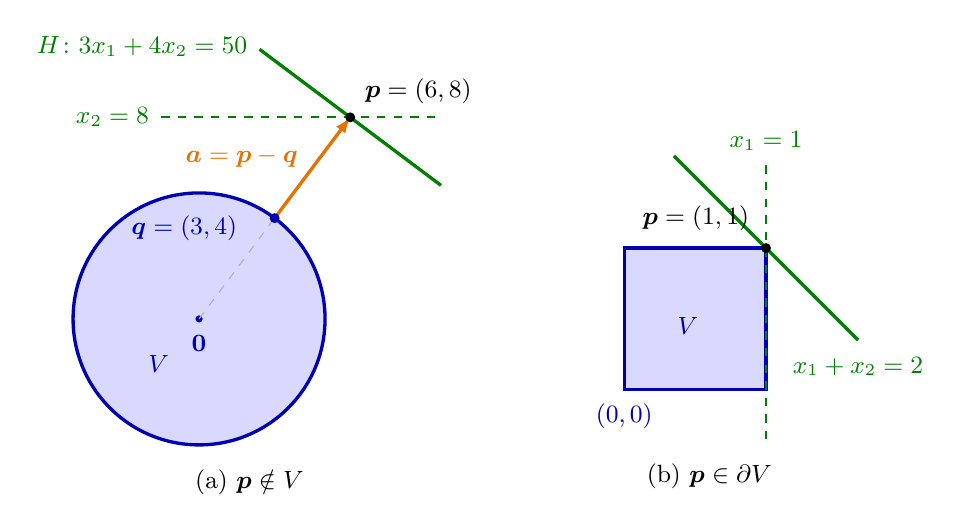
\begin{tikzpicture}[font=\small, >={Latex[length=2mm]}]
  % ---------- (a) point outside a disc ----------
  \begin{scope}[x=0.32cm, y=0.32cm]
    \fill[blue!15] (0,0) circle (5);
    \draw[blue!70!black, very thick] (0,0) circle (5);
    \node[blue!70!black] at (-1.6,-1.8) {$V$};
    \fill[blue!70!black] (0,0) circle (1.3pt);
    \node[blue!70!black, anchor=north] at (0,-0.25) {$\boldsymbol{0}$};
    \draw[gray!60, dashed] (0,0) -- (3,4);
    % alternative hyperplane x2=8
    \draw[green!50!black, thick, dashed] (-1.5,8) -- (9.5,8);
    \node[green!50!black, anchor=east] at (-1.6,8) {$x_2=8$};
    % H: 3x1+4x2=50 through p
    \draw[green!50!black, very thick] (2.4,10.7) -- (9.6,5.3);
    \node[green!50!black, anchor=east] at (2.3,10.8) {$H\colon 3x_1+4x_2=50$};
    % a = p - q
    \draw[orange!90!black, very thick, ->] (3,4) -- (6,8);
    \node[orange!90!black, anchor=east] at (4.3,6.4) {$\boldsymbol{a}=\boldsymbol{p}-\boldsymbol{q}$};
    \fill[black] (6,8) circle (1.8pt);
    \node[anchor=south west] at (6.2,8.15) {$\boldsymbol{p}=(6,8)$};
    \fill[blue!70!black] (3,4) circle (1.8pt);
    \node[blue!70!black, anchor=east] at (1.9,3.6) {$\boldsymbol{q}=(3,4)$};
    \node[anchor=north] at (2,-5.6) {(a) $\boldsymbol{p}\notin V$};
  \end{scope}
  % ---------- (b) boundary point of a square ----------
  \begin{scope}[shift={(5.4cm,-0.9cm)}, x=1.8cm, y=1.8cm]
    \fill[blue!15] (0,0) rectangle (1,1);
    \draw[blue!70!black, very thick] (0,0) rectangle (1,1);
    \node[blue!70!black] at (0.45,0.45) {$V$};
    \node[blue!70!black, anchor=north] at (0,-0.03) {$(0,0)$};
    \draw[green!50!black, thick, dashed] (1,-0.35) -- (1,1.6);
    \node[green!50!black, anchor=south] at (1,1.62) {$x_1=1$};
    \draw[green!50!black, very thick] (0.35,1.65) -- (1.65,0.35);
    \node[green!50!black, anchor=north] at (1.65,0.3) {$x_1+x_2=2$};
    \fill[black] (1,1) circle (1.8pt);
    \node[anchor=south east] at (0.95,1.05) {$\boldsymbol{p}=(1,1)$};
    \node[anchor=north] at (0.6,-0.45) {(b) $\boldsymbol{p}\in\partial V$};
  \end{scope}
\end{tikzpicture}
\end{document}
